\section{Introduction}
A (classical) spin system with $N$ particles is governed by the Edwards-Anderson Hamiltonian 
\begin{align}
	H = -\sum^N_{1\le j < i} J_{ij} s_i s_j,
	\label{eq:connected-Hamiltonian}
\end{align}
with $J_{ij}$ the elements of a 2-dimensional symmetric matrix, dictating the interactions between the particle at the site $i$ and the particle at the site $j$, and $s_i$ is the spin of the particle at the site $i$.
Any two particles interact via a power law
\begin{align}
	J_{ij} \sim \frac{1}{r^{d+\sigma}_{ij}},
\end{align}
with $r_{ij} = \abs{\textbf{r}_i - \textbf{r}_j}$, $d$ the spacial dimensions and $\sigma$ a free parameter characterizing the range of the interaction. 

\textbf{This should appear below, not hoere} The sites are set up in a 1-dimensional chain with periodic boundary conditions, and thus $r_{ij}  = \min( \abs{i - j}, \abs{i-j} - N )$.

\subsection{The Ising model}

\textbf{Notation for states and spins are ambiguous}

A fundamental quantity in statistical mechanics is the partition function \[
	Z = \sum_s \exp (-\beta E_s),
\]
where the sum is performed over states, $\beta =  \frac{1}{T}$ is the inverse temperature and $E_s$ is the energy of the state $s$. By use of the partition function, one is able to calculate observables e.g. the average energy of the system 

\begin{align}
	\begin{split}
	\left< E\right> = 	\sum_s E_s P_s &=  \frac{1}{Z}\sum_s E_s \exp{(-\beta E_s)} \\
									   &= - \frac{1}{Z} \frac{\partial }{\partial \beta } Z \\
									   &= - \frac{\partial \ln Z}{\partial \beta},
	\end{split}
\end{align}
with $P_s$ the probability of finding the system in the state $s$, with energy $E_s$.

The averaging over states is however very computationally expensive, as it is to be summed over the $2dN$ dimensional phase space, with $d$ the dimensions of the configuration space. One instead calculates thermal averages by use of an algorithm by \cite{Metropolis1953}, where the thermal average of an observable $A$ is calculated by generating a sequence of $M$ configurations $\{ s_1, \ldots, s_M \}$ and calculating  
\begin{align}
	\left<A \right> = \frac{1}{M} \sum_{m=0}^M A_m.
\end{align}
A configuration $s_j$  is generated with a probability $\pi_{ij}$ from a configuration $s_i$. The algorithm proposed by \cite{Metropolis1953} relies on the sampling of the state $s_j$ with an \textit{a priori} probability  $\alpha_{ij}$, and it is accepted with a probability $P_{ij}$. While $\alpha_{ij}$ is set by the system, the acceptance probability is  \begin{align}
	P_{ij} = 
	\begin{cases}
		\exp[-\beta (E_{j}	- E_{i})] & E_j > E_i \\
		1 & E_j \leq E_i. 
	\end{cases}
	\label{eq:acceptance-probability}
\end{align}

This way, a new state $s_j$ is always accepted if it lowers the total energy of the system, but also accepts states of total higher energy with a probability that decreases with the temperature.

The simplest case that allows one to study the formation of spontaneous magnetization of ferromagnetic systems is the ising model, where only interaction between nearest neighbors is considered. This is modeled by the Hamiltonian
\begin{align}
	H  = - J \sum_{\left<ij \right>}^N s_{i}s_{j}.
\end{align} 
Here $\left ij \right>$ represents the nearest neighbors of the site $i$, and $J$ is a real constant. In terms of the Hamiltonian \eqref{eq:connected-Hamiltonian}, 
\begin{align}
	J_{ij} = 
	\begin{cases}
	J & i ~\& ~j ~\text{neighbors} \\	
	0 & \text{else}.
	\end{cases}
\end{align} For the Ising model, at each iteration $m$, a new state $s_{m+1}$ is proposed by flipping the spin at a random site with a probability $\alpha_{ij} = N^{-1}$.  The change in energy of the total system depends only on the spins at the nearest neighbors of the site $i.$ By calculating the change in energy, the the new configuration $s_{m+1}$ is accepted with a probability $P_{ij}$ given by \eqref{eq:acceptance-probability}.

However, the Ising model presents no phase transition \cite{ising1925beitrag} for 1-dimensional spin chains, unless long-range interactions are allowed. In order to study the fully connected spin chain with long range interactions \eqref{eq:connected-Hamiltonian}, one needs to compute $\mathcal{O}(n^2)  $ at each iteration $m$ of the Metropolis algorithm. In the interest of reducing this computation time, a mode dilution approximation is proposed.

\subsection{Mode dilution}%
\label{sub:Mode dilution}

The mode dilution approximation studies the Hamiltonian given by \eqref{eq:connected-Hamiltonian}, by setting all the interaction strengths to a constant $J$, and only allowing $N_l$ pairs of sites to interact\footnote{Thus, $J_{ij}$ will have $2N_l$ non-zero elements.}, any two pair of sites ${ i, j } $ is connected with a probability (without normalising) of $r_{ij}^{-(d+\sigma)}$. Figure \ref{fig:a-partially-connected-graph} displays two examples of partially connected graphs with the same $\sigma= 5$, but $N=N_l=10$ for the left panel, and  $N = N_l = 100$ for the  right panel. Both of these graphs present the same coordination number $$z = 2 \frac{N_l}{N},$$ i.e. the average number of bonds (both in- and outgoing) for each node.

\begin{figure}[t]
	\begin{subfigure}{0.5\textwidth}
	\centering
	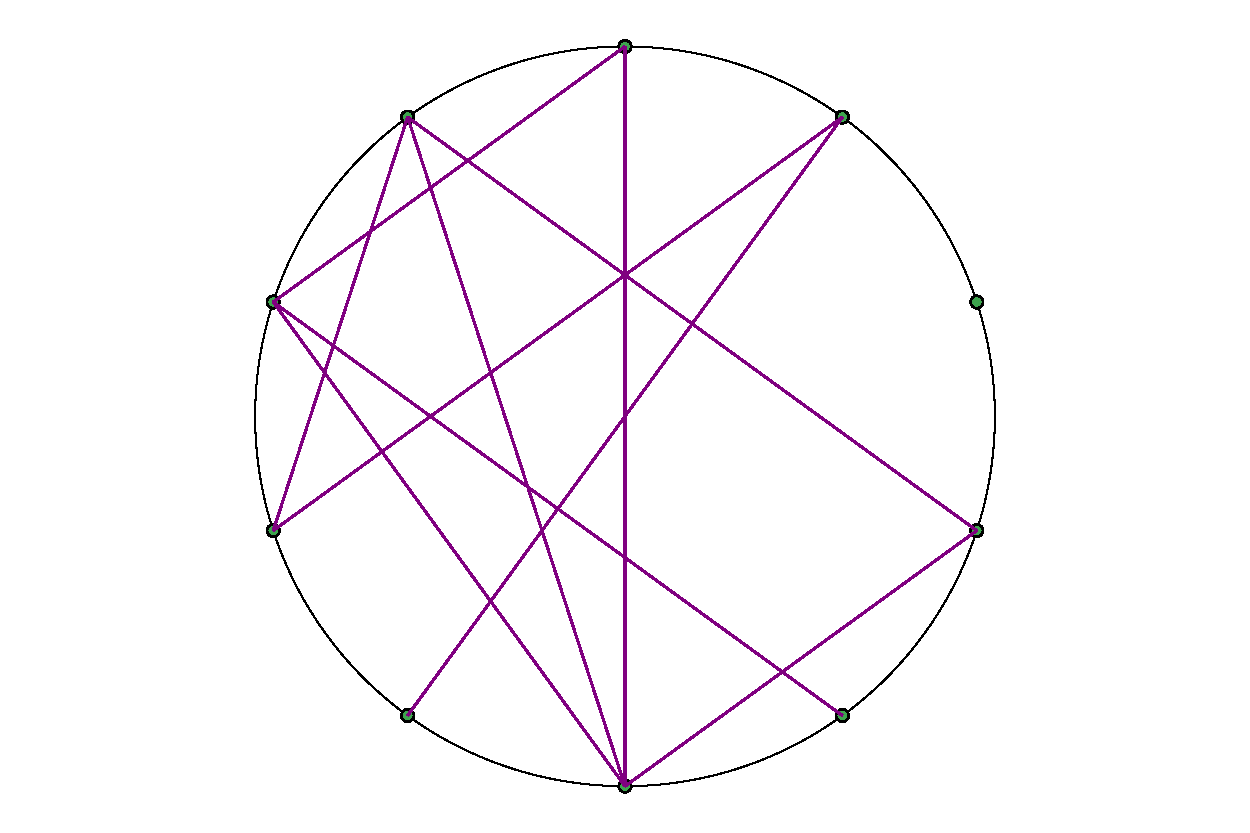
\includegraphics[width=\textwidth]{figures/partially-connected-graph.pdf}
\end{subfigure}
	\begin{subfigure}{0.5\textwidth}
	\centering
	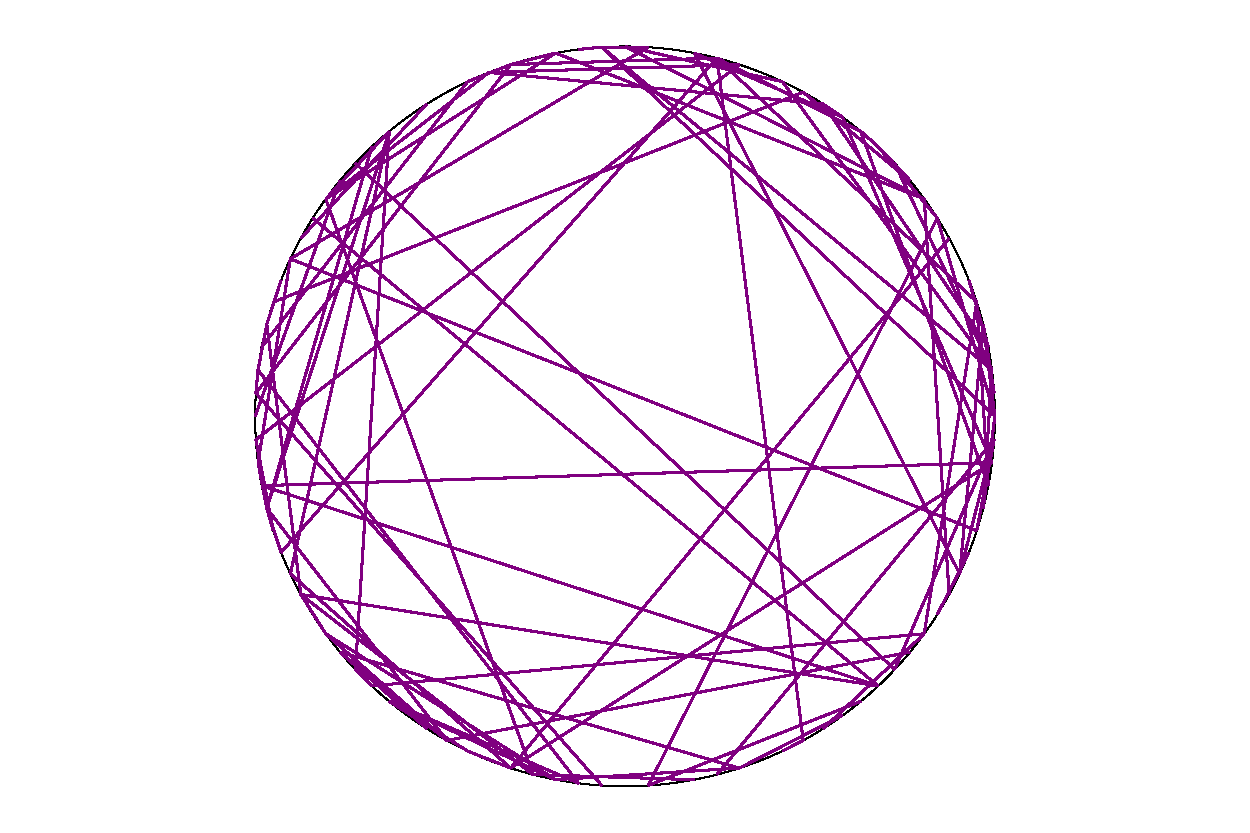
\includegraphics[width=\textwidth]{figures/partially-connected-graph-many-points-nPoints-100-nBonds-100-sigma-5.pdf}
\end{subfigure}
	\caption{Partially connected graphs of different N and $N_l$, but same $\sigma=5$. In the left panel, $N=N_l=10$, and in the right panel $N=N_l=100$.}
	\label{fig:a-partially-connected-graph}
\end{figure}

%Simulations of these systems are very computationaly expensive, as at each `time-step', calculations are of complexity $\mathcal{O}(N^2)$. 
%	A usual simplification of such problems is the Ising model, in wh/kjich the sum in \eqref{eq:connected-Hamiltonian} is performed only over nearest neighbors, which only approximates short-range interactions. The Ising Hamiltonian is \cite{Luijten2006} 
%\begin{align*}
%	\mathcal{H}_{\text{Ising}} = - J \sum_{\langle ij \rangle}^{N} s_i s_j
%,\end{align*}
%where $J$ is now a constant.
%This model is in a sense uninteresting, as it has been shown that 1-dimensional spin glasses with finite non-zero $J_{ij}$ (e.g. the Ising model) does not present phase transitions \cite{Rushbrooke_Ursell_1948}. Long range interactions however, have been found to present phase transitions \cite{Kotliar1983}.
%
%In order to study long range interactions and avoid the $\mathcal{O}(N^2)$ computational cost of computing every interaction, a dilute spin model is used \cite{Leuzzi2008}.
%In this model, the interaction $J_{ij}$ is set distance independent, but the probability of having an interaction decays with $
%	\frac{1}{r^\sigma_{ij}}.$ The coordination number is fixed, and therefore so is the total number of bonds $N_l \leq \frac{N(N-1)}{2}$.

\subsection{Set up}%
\label{sub:Set up}

We consider a 1-dimensional spin-chain with periodic boundary conditions, so that the distance between any two nodes $i, j$, is the minimum distance along the circle that joins them, $r_{ij} = \min(\abs{i - j}, \abs{i-j} - N)$
